\addtocontents{toc}{\protect\setcounter{tocdepth}{2}}
%La ligne ci dessus permet de masquer les subsections de l'intro dans la ToC

\section{Introduction}

\subsection{La Cryptographie}

\begin{frame}
\frametitle{Introduction}
    \begin{tikzpicture}[pin distance=1cm,every pin/.append style={font=\sffamily\itshape}]
    \node[alice,minimum size=2cm,pin={[text width=2em]40:{$\operatorname{enc}$}}] (A) at (2,2) {Alice};
    \node[bob,mirrored, minimum size=2cm,pin={[text width=2em]140:{$\operatorname{dec}$}}] (B) at (10,2) {Bob};
    \node[criminal,female,minimum size=2cm] at (6,-0.5) {Eve};
    \draw [thick,->] (A) -- (B) node[midway,above] {Message secret};
    \end{tikzpicture}
\end{frame}

\begin{frame}{Histoire}
    \startchronology[startyear=1910,stopyear=2019,color=gray,height=7ex,width=\hsize,startdate=false, stopdate=false]
    \chronoperiodecoloralternation{brown,rougeb}
    \chronoperiode[startdate=false, stopdate=false]{1910}{1950}{Cryptographie symétrique}
    \chronoperiode[stopdate=false]{1950}{2019}{Cryptographie asymétrique}
    \chronoevent[markdepth=25pt]{1978}{Invention du RSA}
    \chronoevent[markdepth=50pt]{2009}{Thèse de Craig Gentry}
    \stopchronology
\end{frame}

\subsection{La Cryptographie homomorphe}

\begin{frame}
\frametitle{La cryptographie homomorphe}

\begin{figure}
\begin{tikzpicture}

\node[alice, minimum size=2.1cm, xshift=-1.5cm] at (0, 2) {Alice};

\draw [->] (0, 2) -- (4,2);
\node [above] at (2,2) {Entrées chiffrées};

\draw [->] (4,1) -- (0,1);
\node [below] at (2,1) {Résultat chiffré};

\node[bob, monitor, mirrored, minimum size=2.1cm, xshift=1.75cm] at (5, 2) {Bob};
\node [above] at (6,4) {Gros calculs};

\end{tikzpicture}
\end{figure}

\end{frame}

\begin{frame}{La cryptographie homomorphe}

\begin{alertblock}{Définition : Calculer sur des chiffrés}
Si $m$ est un mot \textbf{clair}, $c = \operatorname{enc}(m)$ son \textbf{chiffré}, et $f$ une fonction, $f$ est \textbf{compatible} pour le schéma si
    $$\operatorname{dec}(f(c)) = f(m)$$
\end{alertblock}

\begin{alertblock}{En pratique} % Bloc alerte rouge
\textbf{Somme} et \textbf{produit} car \textbf{polynôme}
\end{alertblock}
    
\end{frame}

\begin{frame}{La cryptographie homomorphe}

\begin{alertblock}{Définition : Cryptographie partiellement homomorphe}
On peut effectuer des additions \textbf{et/ou} des multiplications en nombre \textbf{fini}
\end{alertblock}

\begin{alertblock}{Définition : Cryptographie complètement homomorphe}
On peut effectuer des additions \textbf{et} des multiplications en nombre \textbf{infini} 
\end{alertblock}

\begin{alertblock}{Pourquoi fait on la distinction ?}
La cryptographie homomorphe se base sur du \textbf{bruit}.
\end{alertblock}

\end{frame}

\begin{frame}{La cryptographie homomorphe}
    \begin{center}
    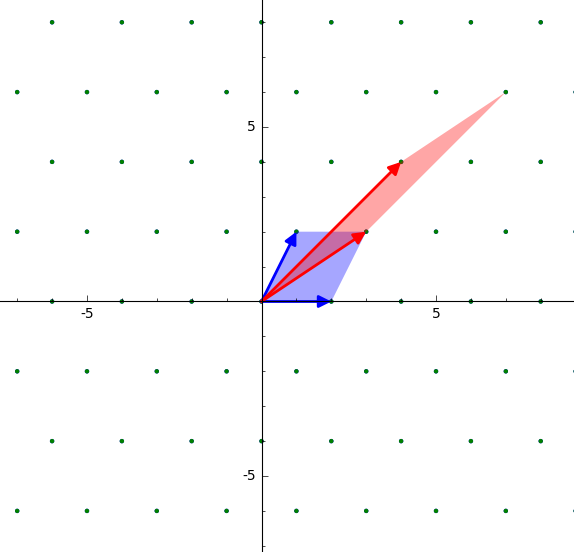
\includegraphics[scale=0.43]{images/exemple_reseau2.png} 
    \end{center}
\end{frame}{}

\begin{frame}{État de l'art}
    \begin{alertblock}{Avant la Thèse de Craig Gentry}
    Cryptographie \textbf{partiellement homomorphe}
    \end{alertblock}
    \begin{alertblock}{Thèse de Craig Gentry (2009)}
    Astuce : \textbf{bootstrap}
    \end{alertblock}
    \begin{alertblock}{Depuis la thèse de Craig Gentry}
        Beaucoup de schémas \textbf{théoriques}\\
        Aucune application concrète car \textbf{aucun n'est assez performant}
    \end{alertblock}{}
\end{frame}{}


\addtocontents{toc}{\protect\setcounter{tocdepth}{2}}

%fin de l'introduction : rajouter le schéma va-et-vient  + finir l'etat de l'art